%!TEX root = ../Peerbox.tex



\subsection{Middleware}
communication between peers via multicast 

however ip multicast is per se unreliable, early test have shown a miss rate of 20\%

negative acknowledgements

reliable multicast

additional checksum to verify payload

\subsubsection{Message}

%figure message package

command can be either Message (1), ACK(2) or NACK(4). 
Acks are not used in this implementation in order to reduce traffic on the channel 

the size of the payload is dynamic though it is not allowed to be larger than the maximum message size, which is in our case preset to $2^15$. A fixed message size is important in order to determine the number of sizes from incoming messages. 


However, if the logic needs to send a lot of data, it can be split onto multiple messages (due to the reliable multicast it is guaranteed that all messages will eventually arrive and are consumed in order).



\begin{figure}[htbp]
    \centering
        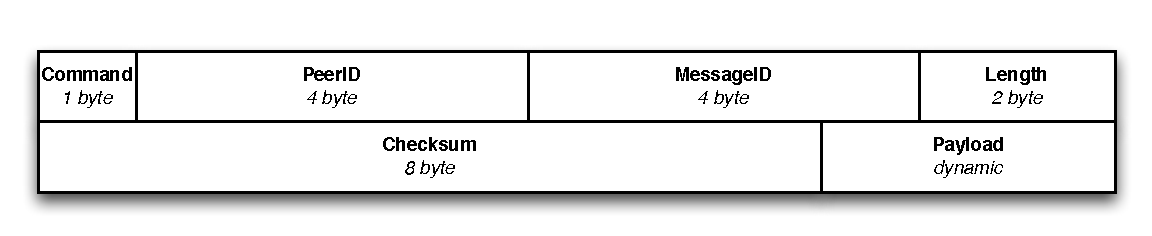
\includegraphics[width=.9\textwidth]{figures/message.pdf}
    \caption{caption}
    \label{fig:figures_announcement}
\end{figure}

use of resources  is indicated by a dashed line 
processes are divided by swim-lanes (dotted vertical lines)

\begin{figure}[htbp]
    \centering
        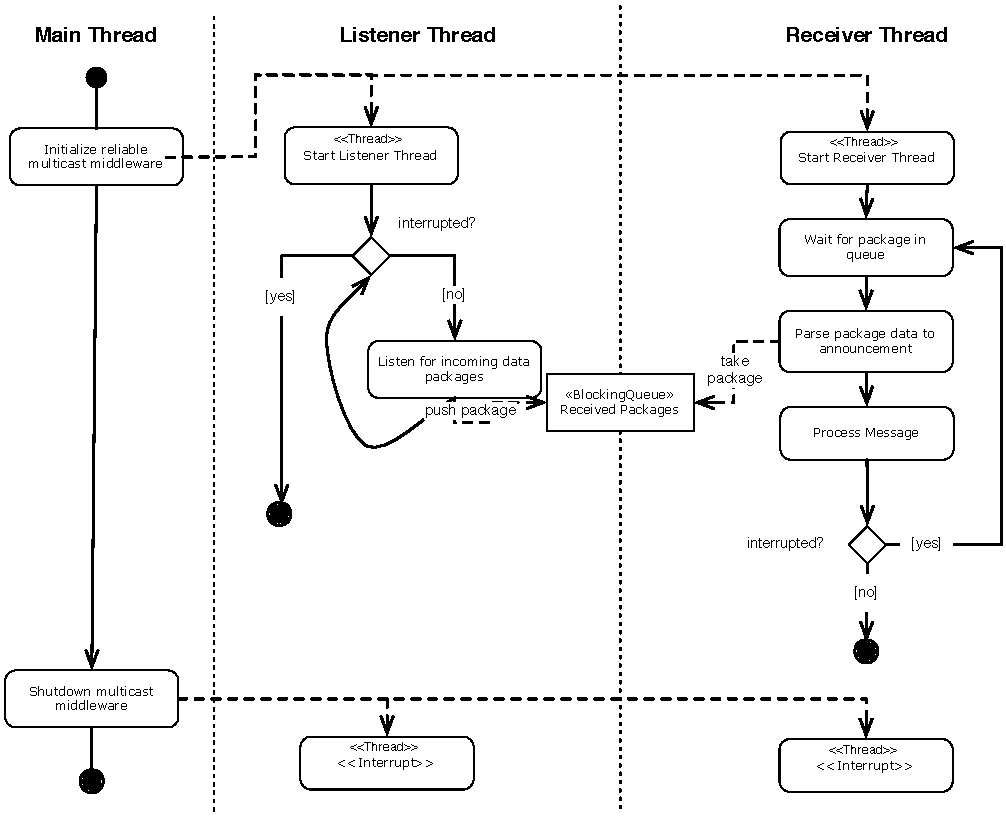
\includegraphics[height=4in]{figures/receivePackets.pdf}
    \caption{Message}
    \label{fig:figures_processReceivePackage}
\end{figure}

\begin{figure}[htbp]
    \centering
        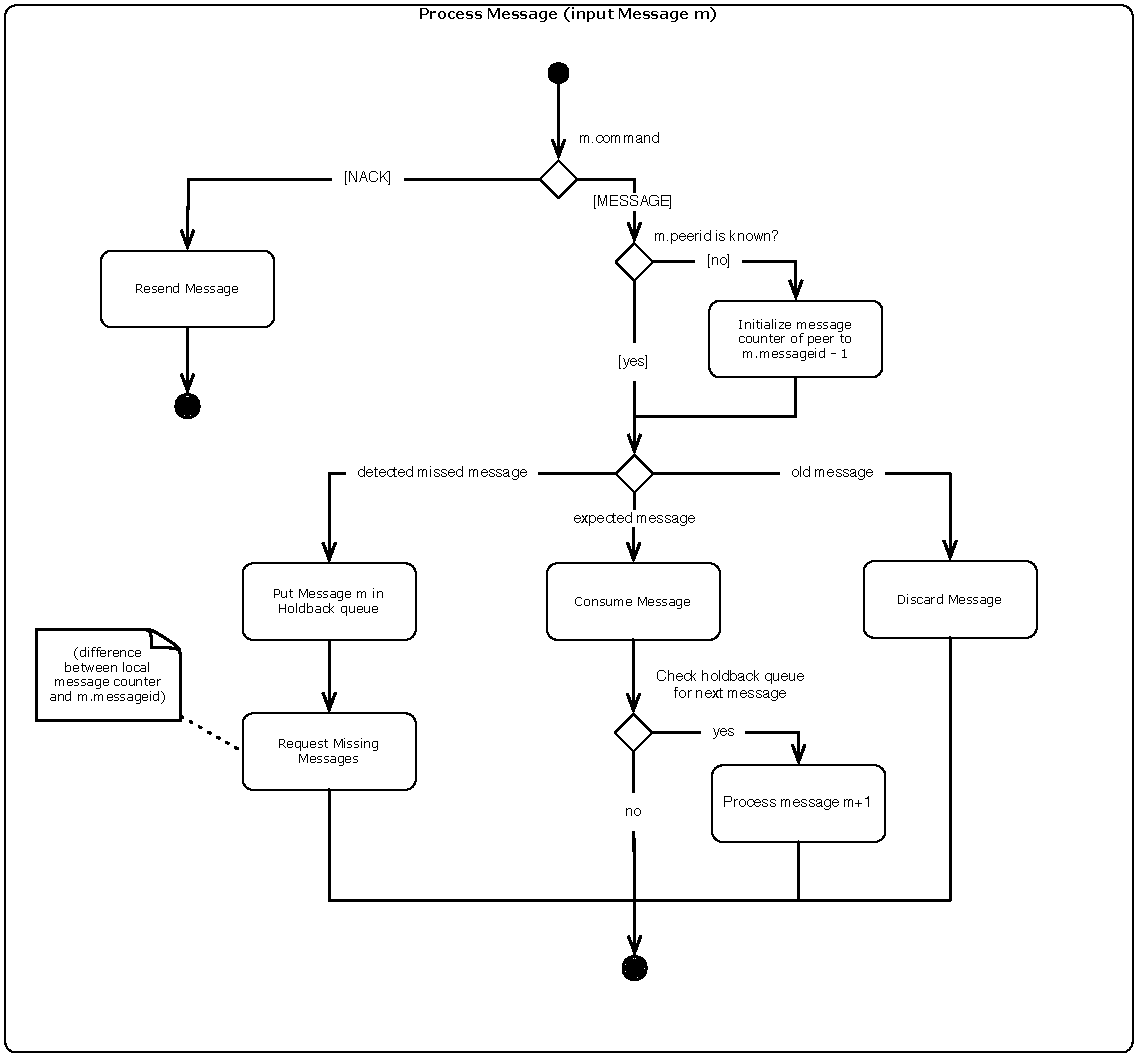
\includegraphics[height=4in]{figures/processMessages.pdf}
    \caption{caption}
    \label{fig:figures_processMessages}
\end{figure}

\begin{figure}[htbp]
    \centering
        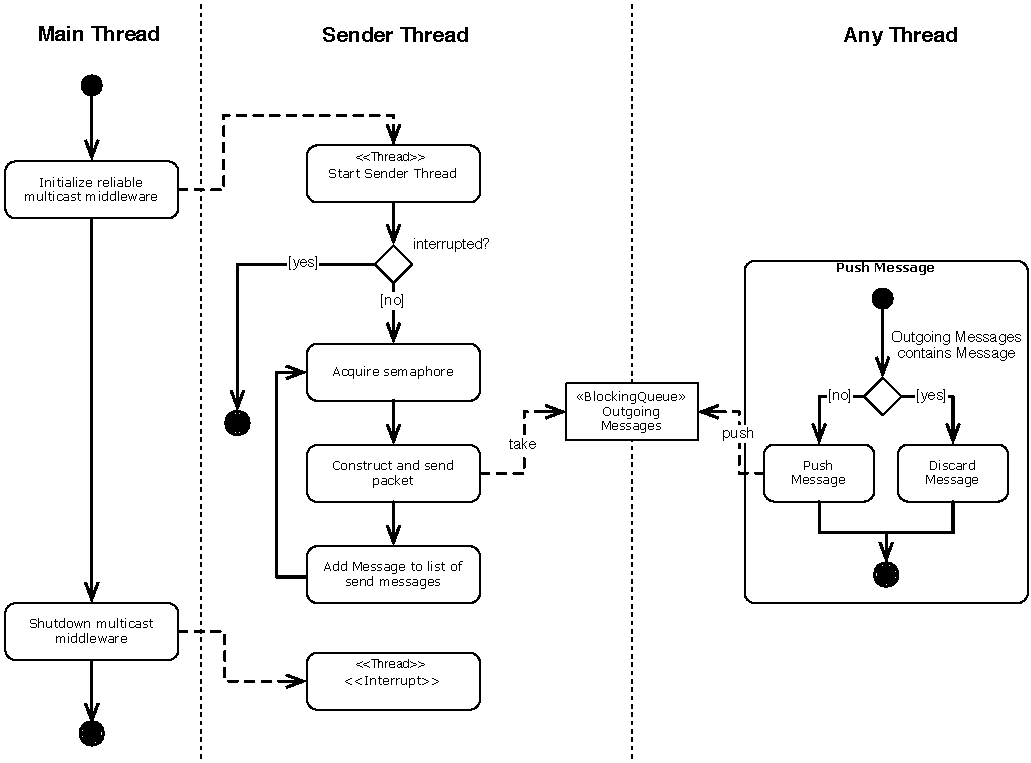
\includegraphics[height=4in]{figures/sendMessage.pdf}
    \caption{caption}
    \label{fig:figures_processMessages}
\end{figure}

\subsubsection{Optimizations}

limit bandwidth 
    - should be made dynamic
    
queue optimizations (discard duplicate)

\subsection{Logic}


\subsection{Interface}